\documentclass[11pt,a4paper]{article}
\usepackage[margin=1in]{geometry}
\usepackage{amsmath,amssymb}
\usepackage{booktabs}
\usepackage{hyperref}
\usepackage{enumitem}
\usepackage{xcolor}
\usepackage{float}
\usepackage{tikz}
\usepackage{pgfplots}
\pgfplotsset{compat=1.18}

% Define custom colors
\definecolor{darkred}{RGB}{180,0,0}
\definecolor{darkblue}{RGB}{0,0,180}

\title{\textbf{Multi-Layer Perceptrons \& Backpropagation}}
\author{Raj K Jain \\ Roll Number: 2025201036}
\date{}

\begin{document}
\maketitle
\vspace{-0.5em}
\noindent\textit{Question: Explain why the hypothesis space explored by gradient-descent-based backpropagation depends on initialization. Discuss how different initializations can lead to different local minima and different learned functions.}

\section*{1. Conceptual Explanation: Intuition}
In machine learning, a model's ``hypothesis space'' is the theoretical set of all possible functions it can learn to map inputs to outputs. Because Multi-Layer Perceptrons (MLPs) with non-linear activation functions are universal approximators, their theoretical hypothesis space is massive. However, we do not explore this space randomly; we navigate it using gradient descent via backpropagation.

The loss landscape of a deep neural network is highly non-convex, resembling a vast, multidimensional mountain range filled with millions of valleys (local minima), ridges (saddle points), and flat plains. Gradient descent is fundamentally a greedy, local search algorithm---much like dropping a ball onto this mountain range and letting gravity pull it down the steepest slope. The exact coordinate where you drop the ball---the initial weights of the network---determines which valley it will ultimately roll into. Therefore, the \textit{effective} hypothesis space explored by the network is completely constrained by its starting point. Two identical networks initialized with different random weights will travel completely different mathematical trajectories, settle into different local minima, and ultimately learn two distinct functional representations of the exact same data.

\section*{2. Mathematical Core: The Symmetry Trap}
To demonstrate how strictly initialization governs the reachable hypothesis space, we can examine the classic ``Symmetry Problem'' that occurs if weights are initialized poorly (e.g., initialized to zero or a uniform constant).

\subsection*{2.1 The Symmetry Problem}
Suppose we have an MLP with one hidden layer containing two neurons, $h_1$ and $h_2$, connected to a single input $x$ and output $y$. Let their respective weights be $w_1$ and $w_2$. If we initialize $w_1 = w_2 = 0$, both neurons compute the exact same output during the forward pass: $h_1 = h_2$.

During backpropagation, the loss gradient with respect to each weight relies on the neuron's activation. Because the activations are perfectly identical, the computed gradients will also be perfectly identical:
$$ \frac{\partial L}{\partial w_1} = \frac{\partial L}{\partial w_2} $$

When the optimizer updates the weights using learning rate $\eta$:
$$ w_1^{(t+1)} = w_1^{(t)} - \eta \frac{\partial L}{\partial w_1} $$
$$ w_2^{(t+1)} = w_2^{(t)} - \eta \frac{\partial L}{\partial w_2} $$

Because both the initial weights and the gradients are equal, the updated weights $w_1^{(t+1)}$ and $w_2^{(t+1)}$ remain exactly equal. By choosing a uniform initialization, we mathematically trapped the network in a severely restricted subspace. The network behaves exactly like a single-neuron network, permanently destroying its capacity to learn complex, multi-featured functions.

\subsection*{2.2 Numerical Example: Weight Evolution with Poor Initialization}
To make this concrete, consider the following numerical dry-run. Suppose on a given training iteration, we compute the same gradient for both neurons: $\frac{\partial L}{\partial w_1} = \frac{\partial L}{\partial w_2} = 0.05$. Using learning rate $\eta = 0.1$, we track weight updates:

\begin{center}
\begin{tabular}{|c|c|c|c|}
\hline
\textbf{Iteration} & $w_1^{(t)}$ & $w_2^{(t)}$ & Update $-\eta \cdot \frac{\partial L}{\partial w_i}$ \\
\hline
0 (Init) & 0.00 & 0.00 & -0.005 \\
\hline
1 & -0.005 & -0.005 & -0.005 \\
\hline
2 & -0.01 & -0.01 & -0.005 \\
\hline
3 & -0.015 & -0.015 & -0.005 \\
\hline
\end{tabular}
\end{center}

Notice that $w_1^{(t)}$ and $w_2^{(t)}$ remain perfectly synchronized throughout training. The network has effectively collapsed to representing a single neuron with weight $w$, unable to learn any interaction or difference between the two hidden units. This symmetry persists indefinitely---no amount of training can break it. In contrast, if we initialize $w_1 = 0.02$ and $w_2 = -0.03$ (asymmetric), the two neurons receive identical gradients but start from different points, allowing them to diverge and learn specialized representations.

\subsection*{2.3 Impact on Hypothesis Space}
The reachable set of functions is thus restricted to those representable by a \emph{single} hidden neuron rather than two. The dimensionality of the effective hypothesis space has been artificially reduced from the theoretical maximum. This illustrates the fundamental principle: \textbf{initialization acts as a hard constraint on the regions of weight space reachable by gradient descent}. Once the network is locked into symmetric weights, no amount of gradient information can escape, regardless of how well-designed the optimizer is.

\section*{3. Visual Element: 3D Loss Landscape}
The 3D surface plot below illustrates a non-convex loss function $L(w_1, w_2)$ parameterized by two weights. Unlike a convex function which acts as a single global bowl, deep learning loss landscapes have multiple valleys. The red and blue markers represent two different random initializations. Because they begin on different slopes of the hyper-surface, their respective gradients pull them into completely isolated local minima.

\begin{figure}[H]
\centering
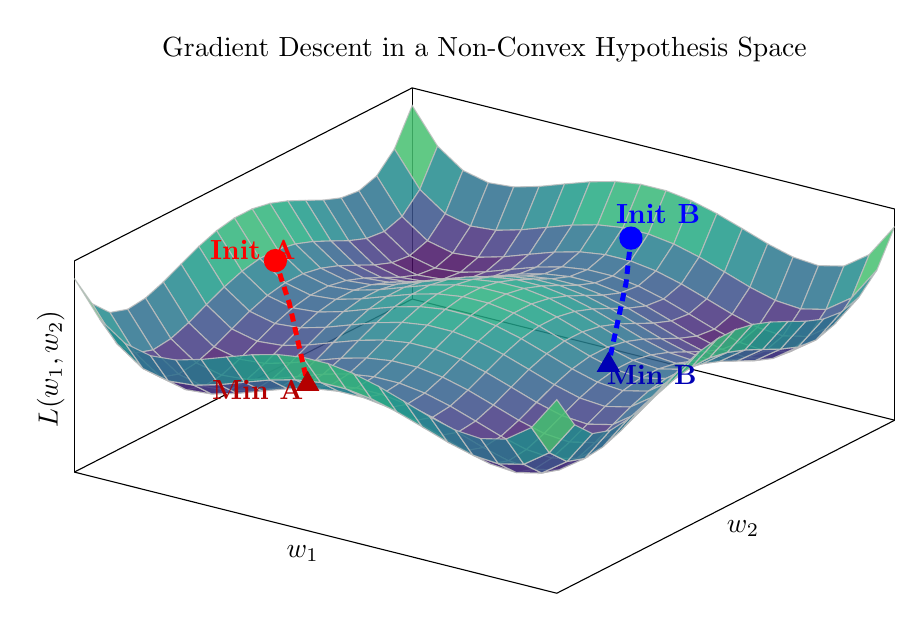
\begin{tikzpicture}
\begin{axis}[
    colormap/viridis,
    view={35}{45},
    xlabel={$w_1$},
    ylabel={$w_2$},
    zlabel={$L(w_1,w_2)$},
    xtick=\empty,
    ytick=\empty,
    ztick=\empty,
    width=12cm,
    height=8cm,
    grid=major,
    title={Gradient Descent in a Non-Convex Hypothesis Space}
]
    % Reduced samples=20 (from 40) to prevent compile timeout
    \addplot3[
        surf,
        domain=-1.5:1.5,
        domain y=-1.5:1.5,
        samples=20,
        opacity=0.85,
        faceted color=black!25
    ] {x^4 + y^4 - 2*x^2 - 2*y^2 + 4};

    % Trajectory A: Init A -> Min A
    \addplot3[red, line width=1.8pt, densely dashed] coordinates {
        (-1.3, 0, 3.5)
        (-1.2, -0.02, 2.5)
        (-1.1, 0, 0.4)
    };

    % Trajectory B: Init B -> Min B
    \addplot3[blue, line width=1.8pt, densely dashed] coordinates {
        (0, 1.3, 3.5)
        (0.04, 1.2, 2.5)
        (0, 1.1, 0.4)
    };

    % Minima markers
    \addplot3[mark=triangle*, mark size=4.5, color=darkred]  coordinates {(-1.1, 0, 0.4)};
    \addplot3[mark=triangle*, mark size=4.5, color=darkblue] coordinates {(0, 1.1, 0.4)};

    % Init markers
    \addplot3[mark=*, mark size=4, color=red]  coordinates {(-1.3, 0, 3.5)};
    \addplot3[mark=*, mark size=4, color=blue] coordinates {(0, 1.3, 3.5)};

    % Labels
    \node[red,  font=\bfseries] at (axis cs:-1.3,-0.2,4.1) {Init A};
    \node[blue, font=\bfseries] at (axis cs:0.1, 1.4, 4.1) {Init B};
    \node[darkred,  font=\bfseries] at (axis cs:-1.2,-0.3,0.6) {Min A};
    \node[darkblue, font=\bfseries] at (axis cs:0.2, 1.2, 0.2) {Min B};

\end{axis}
\end{tikzpicture}
\caption{3D non-convex loss landscape with two distinct local minima. Red and blue trajectories show gradient descent paths from different initializations (circles) to their respective local minima (triangles), illustrating how initialization constrains the reachable hypothesis space.}
\end{figure}

\section*{4. Connections}
This concept connects directly to our study of \textbf{Optimizers (like Adam and SGD with Momentum)} from Module 1. While initialization dictates the starting basin in the loss landscape, advanced optimizers alter how we explore that specific local region. For instance, momentum can provide the ``velocity'' needed to escape a shallow local minimum that a poor initialization might have dropped us into, allowing the model to reach a deeper, wider, and better-generalizing minimum nearby. However, even with momentum, the final learned function is still heavily tethered to the general region dictated by the initial weights.

\section*{5. References}
\begin{itemize}
    \item Goodfellow, I., Bengio, Y., \& Courville, A. (2016). \textit{Deep Learning} (Chapter 8: Optimization for Training Deep Models). MIT Press.
    \item Course Lectures: \textit{Statistical Methods in Artificial Intelligence}, Spring 2026, Module 2 (Neural Networks).
    \item Wikipedia. (2024). Backpropagation --- Symmetry Problem. Retrieved from \url{https://en.wikipedia.org/wiki/Backpropagation#Symmetry_problem}
    \item Wikipedia. (2024). Weight Initialization --- Symmetry Problem. Retrieved from \url{https://en.wikipedia.org/wiki/Weight_initialization#Symmetry_problem}
\end{itemize}

\end{document}